\section*{Описание структур данных}

\subsection*{Список}

Для хранения данных о грузовиках используется линейный двусвязный список.
Схема списка представлена на рис.\ref{list_schema}.

\begin{figure}[htp!]
    \centering
    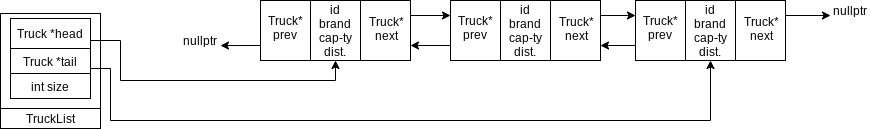
\includegraphics[width=0.9\linewidth]{photo/list_schema}
    \caption{Схема списка}
    \label{list_schema}
\end{figure}

\subsection*{Структуры}

Грузовик Truck представлен в памяти программы в виде структуры с следующими полями:

\begin{itemize}
    \item \verb|int id;| -- идентификатор грузовика
    \item \verb|float capacity;| -- максимальна масса груза
    \item \verb|int transportation\_distance;| -- дальность перевозки
    \item \verb|std::string brand;| -- марка
    \item \verb|Truck *prev;| -- указатель на предыдущий элемент
    \item \verb|Truck *next;| -- указатель  на следующий элемент
\end{itemize}

Структура для работы с элементами списка TruckList сожержит следующие поля:

\begin{itemize}
    \item \verb|Truck *head;| -- указатель на первый элемент списка
    \item \verb|Truck *tail;| -- указатель на последний элемент списка
    \item \verb|int size;| -- количество элементов в списке
\end{itemize}

Структура для высокоуровневой работы со списком TruckDataBase сожержит единственное поле:

\begin{itemize}
    \item \verb|TruckList list{};| -- список
\end{itemize}

Для получения команд от пользователя создана структура Cmd с следующими полями:

\begin{itemize}
    \item \verb|Command command = Command::NONE;| -- команда к выполнению
    \item \verb|std::string command\_str{};| -- введённая команда
    \item \verb|const std::string prompt = "LR \$>";| -- приглашение командной строки
    \item \verb|TruckDataBase *tp;| -- указатель на БД, над которой производится выполнение команды
\end{itemize}

Command -- перечисление, содержащее возможные команды.
Состоит из:

\begin{itemize}
    \item \verb|Add| -- добавить элемент в список
    \item \verb|Load| -- загрузить список из файла
    \item \verb|Save| -- сохранить список в файл
    \item \verb|Print| -- напечатать элемент по индексу
    \item \verb|PrintAll| -- напечатать все элементы
    \item \verb|Help| -- справка
    \item \verb|Insert| -- вставить элемент в список
    \item \verb|Delete| -- удалить элемент из списка
    \item \verb|Edit| -- редактировать элемент
    \item \verb|SortByBrand| -- отсортировать список по марке
    \item \verb|SortByCapacity| -- отсортировать список по грузоподъёмности
    \item \verb|SortByDistance| -- отсортировать список по дальности перевозки
    \item \verb|FindByBrand| -- найти элементы по марке
    \item \verb|FindByCapacity| -- найти элементы по грузоподъёмности
    \item \verb|FindByDistance| -- найти элементы по дальности перевозки
    \item \verb|Exit| -- выход
    \item \verb|Skip| -- (пустая команда)
    \item \verb|NONE| -- неопределённая команда
\end{itemize}

Структуры и их взаимосвязи представлены
в виде диаграммы классов на рис.\ref{class_diagram}

\begin{figure}[htp!]
    \centering
    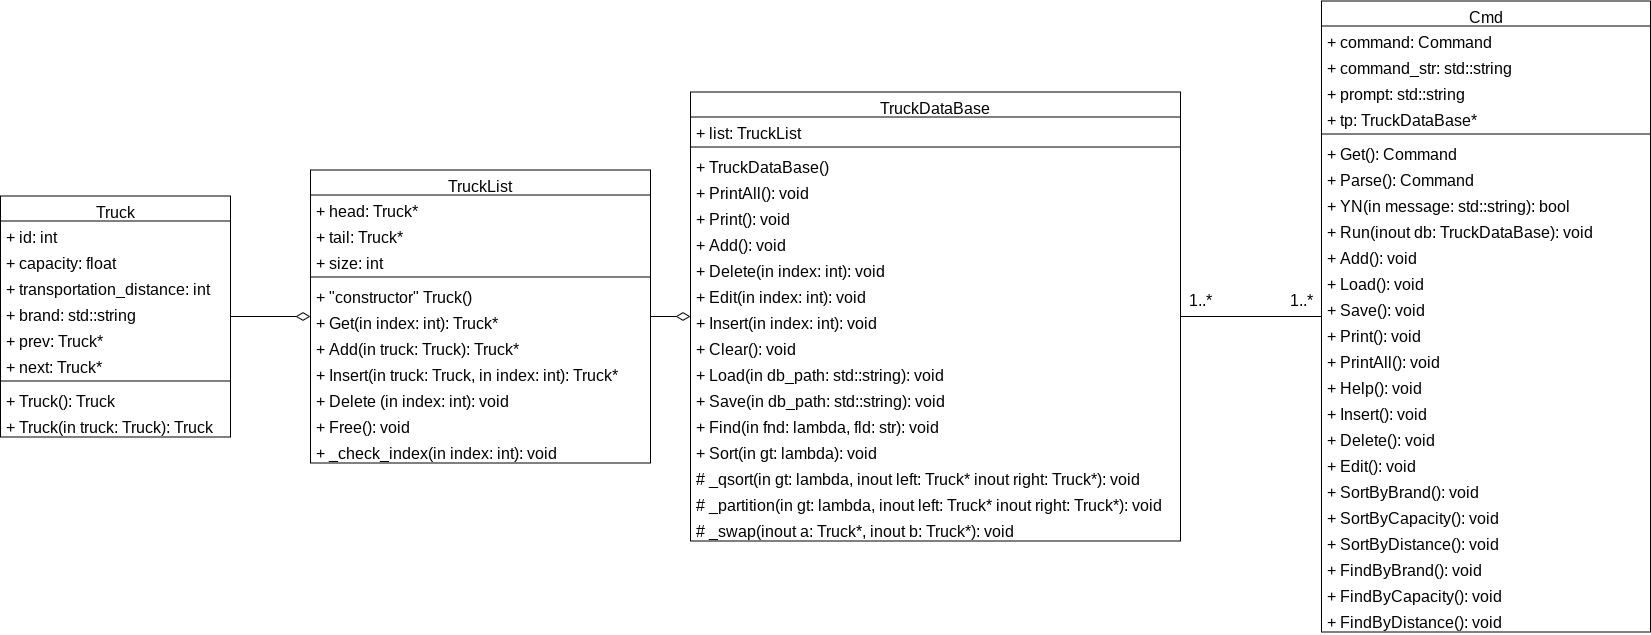
\includegraphics[width=0.9\linewidth]{photo/class_diagram}
    \caption{Диаграмма классов по програмным структурам}
    \label{class_diagram}
\end{figure}